\documentclass[12pt,a4paper]{article}
%%% Packages %%%
\usepackage{algorithm}		% Algorithms with captions (\begin{algorithm}).
\usepackage{algpseudocode}	% Algorithm pseudocode (\begin{algorithmic}).
\usepackage{amsfonts} 		% For extra mathy stuff (\mathbb).
\usepackage{amsmath} 		% For section headers.
\usepackage{amssymb} 		% For extra mathy stuff, e.g. \therefore.
\usepackage{amsthm}  		% Custom theorem styles.
\usepackage[toc,page]{appendix} % Appendices.
\usepackage{array} 			% Special tabular.
\usepackage{braket} 		% For \set \bra \ket commands.
\usepackage{caption} 		% Caption setup.
\usepackage{centernot} 		% For \centernot.
\usepackage{enumitem} 		% For \setlist.
\usepackage[T1]{fontenc} 	% Code blocks!
\usepackage[margin=1in]{geometry} % global page margin
\usepackage{hyperref} 		% For links.
\usepackage[latin1]{inputenc} % For fancy text input
\usepackage{lipsum} 		% Lorem ipsum <3
\usepackage{listings} 		% Code blocks!
\usepackage{longtable} 		% For the longtable env.
\usepackage{mathtools} 		% \DeclarePairedDelimiter
\usepackage{multirow}		%
\usepackage{scrextend} 		% For the ddmargin env.
\usepackage[inference]{semantic} % Logical inference.
\usepackage{setspace} 		% Custom line spacing.
\usepackage{textcomp} 		% Code blocks.
\usepackage{url} 			% URLs in bibliography.
\usepackage{verbatim} 		% Multiline comments.
\usepackage{wrapfig} 		% Text-wrapping around figures.
\usepackage[svgnames]{xcolor} % For some pretty colours; see https://www.latextemplates.com/svgnames-colors.
\usepackage{ulem}  			% For \sout.

\usepackage{graphicx} 		% Graphics~
\graphicspath{{img/}}

\usepackage{booktabs, makecell, tabularx}

% \usepackage{apacite}
\usepackage[sort,comma,nonamebreak]{natbib}
% \bibliographystyle{apalike}
\bibliographystyle{plainnat}
% \bibliographystyle{apacite}


\usepackage{tikz} % Tikz!!!
\usepackage{tikz-qtree} % Simple trees!
\usetikzlibrary{arrows}

\usepackage{fancyhdr} % Um... Fancy headers!
\pagestyle{fancy}

\usepackage{mathptmx} % Times New Romans-esque font.

%%% Tex Commands. %%%

% Side-by-side figures with captions!
% \DeclareCaptionLabelFormat{cont}{#1~#2\alph{ContinuedFloat}}
% \captionsetup[ContinuedFloat]{labelformat=cont}

% Convenience wrapper for bracketing. \delim* for auto-sizing, \delim[\bigg] for manual sizing.
\DeclarePairedDelimiter\ceil{\lceil}{\rceil}
\DeclarePairedDelimiter\floor{\lfloor}{\rfloor}
\DeclarePairedDelimiter\abs{\lvert}{\rvert}
\DeclarePairedDelimiter\parens{(}{)}
\DeclarePairedDelimiter\angles{\langle}{\rangle}

%%%% Useful Macros %%%
\renewcommand{\o}{\varnothing} % Empty set.
\newcommand{\N}{\mathbb{N}} % Natural numbers.
\newcommand{\Z}{\mathbb{Z}} % Integers.
\newcommand{\Q}{\mathbb{Q}} % Rational numbers.
\newcommand{\R}{\mathbb{R}} % Real numbers.
\newcommand{\C}{\mathbb{C}} % Complex numbers.
\newcommand{\powerset}{\mathcal{P}} % Power set.
\newcommand{\insum}{\textstyle\sum} % Inline summation.
\newcommand{\st}{\text{ such that }} % Inline summation.

\renewcommand{\Return}{\State \textbf{return }} % Pseudocode return statement. To be used with the algorithmic package.

\renewcommand{\epsilon}{\varepsilon}
\renewcommand{\b}[1]{\!\left(#1\right)}

\newcommand{\xor}{\oplus}
\newcommand{\cnot}{\centernot}

\DeclareRobustCommand{\abinom}{\genfrac{\langle}{\rangle}{0pt}{}}

\newcommand{\code}[1]{\texttt{#1}}

% \includecode[<caption>]{filename}
\newcommand{\includecode}[2][]{\lstinputlisting[caption=#1, escapechar=, style=custom_python]{#2}}

% Usage:
% \begin{graph}
% 	\node{parent}
%		child {node {child 1}}
% 		child {node {child 2}};
% \end{graph}
\newenvironment{graph}[1]
	{
		\begin{minipage}{#1}
			\centering
			\begin{tikzpicture}
				\tikzset{filled/.style = {shape=circle,fill,minimum size=0.1em}}
				\tikzset{edge/.style = {-,> = latex'}}
				\tikzset{arrow/.style = {->,> = latex'}}
				\tikzset{sibling distance=6em, every node/.style = {shape=circle,draw,minimum size=1em}}
	}
	{
			\end{tikzpicture}
		\end{minipage}
	}

% \newenvironment{tree}[1]
% 	{
% 		\begin{graph}[
% 			sibling distance=10em,
% 			every tree/.style = {shape=rectangle, rounded corners,
% 			  draw, align=center,
% 			  top color=white, bottom color=blue!20}]]
% 			]{#1}
% 	}
% 	{
% 		\end{graph}
% 	}

% Theorems!!!
\newtheorem{theorem}{Theorem}[section]
\newtheorem*{definition*}{Definition}

% Named theorems!
\makeatletter
\newtheoremstyle{namedStyle}
{\topsep}{\topsep}
{}{}
{\bfseries}{.}
{0.5em}
{\thmname{\@ifempty{#3}{#1}\@ifnotempty{#3}{#3}}}
\makeatother
\theoremstyle{namedStyle}
\newtheorem*{solution}{Solution}
\newtheorem*{namedProof}{Proof}

%%% Document Settings %%% 
% Global line spacing.
% \onehalfspacing % 1.5
\doublespacing % 2.0
% \setstretch{1.25} % Custom.

\setlength\parindent{24pt} % Paragraph indent.
\setlength{\headheight}{15pt}

\renewcommand\tabcolsep{5pt} % Table column spacing.
\renewcommand\arraystretch{0.9} % Matrix spacing (or table row spacing).

%%% List Settings %%%
% https://tex.stackexchange.com/questions/300340/topsep-itemsep-partopsep-parsep-what-do-they-each-mean-and-what-about

% \setlist{nosep} % Set tight ordered-lists.

% Default enumerate.
\setenumerate{
	label=(\alph*),
	topsep=1pt,
	itemsep=1pt,
	parsep=1em, % Separation between paragraphs within items.
	}

\makeatletter
% \skipitems{n: int}: skip items in an enumerated list
\newcommand{\skipitems}[1]{%
	\addtocounter{\@enumctr}{#1}%
}

% Same-line enumerated items. Use \inlineitem instead of \item.
% https://tex.stackexchange.com/a/51089/179128
\newcommand{\inlineitem}[1][]{%
\ifnum\enit@type=\tw@
	{\descriptionlabel{#1}}
	\hspace{\labelsep}%
\else
	\ifnum\enit@type=\z@
		\refstepcounter{\@listctr}\fi
	\quad\@itemlabel\hspace{\labelsep}%
\fi}
\makeatother

	
%%% Misc. Settings %%%

% Have table and figure use same counter.
\makeatletter 
\let\c@table\c@figure
% \let\c@lstlisting\c@figure
\makeatother

% Graphics.
\graphicspath{ {../res/} }

% Set code format.

%% Usage:
% \begin{lstlisting}[style=custom_python(, options=...)]
% # Code goes here.
% \end{lstlisting}

\lstdefinestyle{custom_python}{
	backgroundcolor = \color{WhiteSmoke},
	basicstyle = \ttfamily\small,
	breaklines = true,
	commentstyle = \itshape\color{DarkGreen},   % Comment style.
	deletekeywords = {set},
	escapeinside = {\%*}{*)},                   % For adding LaTeX in code.
	extendedchars = true,
	frame = single,
	keepspaces = true,
	keywordstyle = \bfseries\color{blue},
	language = Python,                   		% Change the programming language here!
	morekeywords = {*, ValueError, as},
	numbers = left, 							% Line-numbers (possible values: none, left, right).
	numbersep = 10pt,                   		% Distance between line-numbers and code
	numberstyle=\small\color{DarkGray}, 		% Style used for line-numbers.
	rulecolor = \color{black},
	showstringspaces = false,
	stringstyle = \color{red},
	tabsize = 4,
	upquote = true
}

\renewcommand{\vec}{\mathbf}

\newcommand{\name}{\textit{redacted}}
\newcommand{\sid}{\textit{redacted}}
\newcommand{\itsc}{\textit{redacted}}
\newcommand{\thistitle}{COMP3711 Assignment 5}

\begin{document}
	\lhead{\name}
	\chead{\thistitle}
	\rhead{\sid, \itsc}

\newpage
\section*{Q1}
	Since $T$ is tree, it is acyclic and connected.
	For $e \in E'$ with $e = (u,v)$, removing the edge $e$ would result in $V$ splitting into two disjoint sets of vertices: $U$ and $V - U$, with $u \in U$, $v \in V - U$. Note that $e$ has exactly one endpoint in $U$ and exactly one endpoint in $V - U$.

	Since $T$ is the MST of $G$, so $e$ is the shortest edge connecting $U$ and $V - U$. Suppose a shorter edge $e'$ existed that connected $U$ and $V - U$, with $w(e') < w(e)$. Then $T$ wouldn't be the MST since $w(E' - \{e\} \cup \{e'\}) = w(E') - w(e) + w(e') \le w(E')$. By contradiction, $e$ is the shortest (min cost) edge connecting $U$ and $V - U$.

	Thus, there exists a subset of vertices $S_e = U$ such that $e$ is the min cost edge with exactly one endpoint in $S_e$.

\newpage
\section*{Q2}
	\begin{enumerate}[label=(\Alph*)]
		\item 
		We first construct a DAG for the problem.
		We define vertices $s$, $t$, $X_i$ for $1 \le i \le m$, and $C_j$ for $1 \le j \le n$.
		The (directed) edges of the graph are:
		\begin{itemize}
			\item $(s, C_j)$ (with weight 1) for all $1 \le j \le n$ where $L_j = 1$. This represents the courses that have been taken are available to be matched against the requirements.
			\item $(C_j, X_i)$ (with weight 1) for all $1 \le i \le m$, $1 \le j \le n$ where $X_{i,j} = 1$. This represents the matching of the requirements.
			\item $(X_i, t)$ (with weight $N_i$) for all $1 \le i \le m$. This represents the flow of the minimum number of requirements needed.
		\end{itemize}

		We then run the Ford-Fulkerson Max-Flow algorithm on this graph. If a flow exists where $f(s,t) = \sum N_i$ (i.e. all requirements are satisfied), then that means the student can graduate from the Department of Commuter Silence at Sham-Poobanana University.

		\item 
		The heavy lifting is done by the Ford-Fulkerson Max-Flow algorithm, which runs in $O(|V||E|^2)$ time. The initialisation of the vertices and edges and the checking performed in the end will be considered negligible.

		According to (A), we have $|V| = m + n + 2$ and $|E| \le n + mn + m$. For $|E|$, we can only be certain of the upper bound, which is when $L_j = 1 \forall j$ and $X_i,j = 1 \forall i,j$. This is the extreme case when all edges are present.

		We then have
		\begin{align*}
			O(|V||E|^2) &= O((m+n+2)(n+mn+m)) \\
			&= O((m+n)(n(m+1)+m)) \\
			&= O((2n)(n(m+2))) & m \le n \\
			&= O(2n^2(m+2)) \\
			&= O(n^2m)
		\end{align*}

		Note that we made use of the knowledge that $m \le n$. Assuming that $N_i \ge 1$, it only makes sense for $m \le n$; otherwise there are more requirements than courses and it becomes impossible to complete all requirements.

		\item
		The vertex $s$ represents the start of the flow. It is directly connected only to the courses taken, and with a weight of 1, since each course is only taken once and can only be counted once. This is the outward-flow from $s$, and the capacity is the number of courses taken ($\sum L_j$).

		Each course $C_j$ is linked to zero or more requirements. When running the Ford-Fulkerson Max-Flow algorithm, choosing a path with course $C_j$ and some requirement $X_i$ means that we attempt to register $C_j$ to fulfill said requirement $X_i$. Each course can only be used to fulfill one requirement since the in-degree of each course is at most 1, so due to flow, the out-degree is also at most 1 (or at most the in-degree, to be precise).

		To ensure that the requirements are satisfied, the requirement vertices $X_i$ are directly connected to $t$ with weight $N_i$. When running the algorithm, any path will have capacity 1. Selecting a path will decrement $N_i$ in the residual graph until it reaches 0.

		Finally, we perform the final check to ensure that the flow value $|f|$ equals $\sum N_i$. There may be cases where the flow value is less than $\sum N_i$, in which case this means some requirement was not satisfied. But the max flow algorithm is designed to maximise $f$, so if the flow value is less than $\sum N_i$, then we know there are no other flows that will satisfy the graph, and that the problem can't be solved, or in other words, the student can't graduate from the Department of Commuter Silence at Sham-Poobanana University.
		
	\end{enumerate}

\newpage
\section*{Q3}
	\begin{enumerate}[label=(\alph*)]
		\item 
		\begin{enumerate}[label=(\roman*)]
			\item 
			By the Max-Flow Min-Cut algorithm in the lecture notes, if $f$ is a maximum flow, then we can find a min-cut $c(S, T)$ for some $s-t$ cut $(S, T)$. We first weight all edges with 1. We can determine the min-cut by running the Ford-Fulkerson Max-Flow algorithm followed by BFS on $s$ to determine the min-cut.
			
			\item Note that upon the removing the min-cut edges from $G$, there would be no more $s-t$ path, as required. Why? Since $f$ is a max flow, by the min-cut theorem, the residual graph $G_f$ has no path from $s$ to $t$. The maximising property of the Ford-Fulkerson Max-Flow algorithm ensures that the edge set is minimum. Suppose it wasn't minimum, then another path could be added from $s$ to $t$, and $f$ wouldn't be a max flow.
			
			\item From page 38 of the slides, running BFS uses $O(|E|)$ time. Compound this with the $|E|$ iterations needed by Ford-Fulkerson. Unlike the $O(|V||E|^2)$ implementation of Ford-Fulkerson, paths won't be visited more than once.
		\end{enumerate}

		\item 
		\begin{enumerate}[label=(\roman*)]
			\item 
			For every vertex $v \in V$, create two vertices $v_l, v_r$ in $V'$. Moreover, for every vertex $v \in V - \{s, t\}$, create an edge $(v_l, v_r)$ in $E'$. For every edge $(u, w) \in E$, create an edge $(u_r, w_l)$ in $E'$.

			\item
			If $P$ is an $s-t$ path in $G$ that passes through vertex $v$, then the corresponding path $P'$ in $G'$ is an $s_r - t_l$ path that passes through edge $(v_l, v_r)$.
		\end{enumerate}

	\end{enumerate}

\newpage
\section*{Q4}
	\begin{enumerate}[label=(\alph*)]
		\item \-
		\[
		D^{(2)} =
		\begin{pmatrix}
		0        & 5 & 10 & 11       & 3 & 5  \\
		6        & 0 & 16 & 3        & 5 & 13 \\ 
		\infty & 3 & 0  & \infty & 1 & 3  \\ 
		\infty & 4 & 15 & 0        & 2 & 4  \\ 
		8        & 2 & 7  & 3        & 0 & 2  \\ 
		\infty & \infty  & 5  & 1        & 3 & 0  \\ 
		\end{pmatrix}
		\]

		\[
		D^{(4)} =
		\begin{pmatrix}
		0        & 5 & 10 & 6       & 3 & 5  \\
		6        & 0 & 12 & 3        & 5 & 7 \\ 
		9 & 3 & 0  & 4 & 1 & 3  \\ 
		10 & 4 & 9 & 0        & 2 & 4  \\ 
		8        & 2 & 7  & 3        & 0 & 2  \\ 
		11 & 5  & 5  & 1        & 3 & 0  \\ 
		\end{pmatrix}
		= D^{(8)}
		\]

		\item
		\[
			D^{(1)} =
			\begin{pmatrix}
				0 & 8 & 10 & \infty & 3 & \infty \\
				6 & 0 & 16 & 3 & 9 & \infty \\
				\infty & \infty & 0 & \infty & 1 & \infty \\
				\infty & \infty & \infty & 0 & 2 & 10 \\
				\infty & 2 & \infty & \infty & 0 & 2 \\
				\infty & \infty & 5 & 1 & \infty & 0
			\end{pmatrix}
		\]
		\[
			D^{(2)} =
			\begin{pmatrix}
				0 & 8 & 10 & 11 & 3 & \infty \\
				6 & 0 & 16 & 3 & 9 & \infty \\
				\infty & \infty & 0 & \infty & 1 & \infty \\
				\infty & \infty & \infty & 0 & 2 & 10 \\
				8 & 2 & 18 & 5 & 0 & 2 \\
				\infty & \infty & 5 & 1 & \infty & 0
			\end{pmatrix}
		\]
		\[
			D^{(3)} =
			\begin{pmatrix}
				0 & 8 & 10 & 11 & 3 & \infty \\
				6 & 0 & 16 & 3 & 9 & \infty \\
				\infty & \infty & 0 & \infty & 1 & \infty \\
				\infty & \infty & \infty & 0 & 2 & 10 \\
				8 & 2 & 18 & 5 & 0 & 2 \\
				\infty & \infty & 5 & 1 & 6 & 0
			\end{pmatrix}
		\]
		\[
			D^{(4)} =
			\begin{pmatrix}
				0 & 8 & 10 & 11 & 3 & 21 \\
				6 & 0 & 16 & 3 & 5 & 13 \\
				\infty & \infty & 0 & \infty & 1 & \infty \\
				\infty & \infty & \infty & 0 & 2 & 10 \\
				8 & 2 & 18 & 5 & 0 & 2 \\
				\infty & \infty & 5 & 1 & 3 & 0
			\end{pmatrix}
		\]
		\[
			D^{(5)} =
			\begin{pmatrix}
				0 & 5 & 10 & 8 & 3 & 5 \\
				6 & 0 & 16 & 3 & 5 & 7 \\
				9 & 3 & 0 & 6 & 1 & 3 \\
				10 & 4 & 20 & 0 & 2 & 4 \\
				8 & 2 & 18 & 5 & 0 & 2 \\
				11 & 5 & 5 & 1 & 3 & 0
			\end{pmatrix}
		\]
		\[
			D^{(6)} =
			\begin{pmatrix}
				0 & 5 & 10 & 6 & 3 & 5 \\
				6 & 0 & 12 & 3 & 5 & 7 \\
				9 & 3 & 0 & 4 & 1 & 3 \\
				10 & 4 & 9 & 0 & 2 & 4 \\
				8 & 2 & 7 & 3 & 0 & 2 \\
				11 & 5 & 5 & 1 & 3 & 0
			\end{pmatrix}
		\]
	\end{enumerate}

\newpage
\section*{Q5}
	\begin{enumerate}[label=(\alph*)]
		\item \-
		\begin{figure}[h!]
			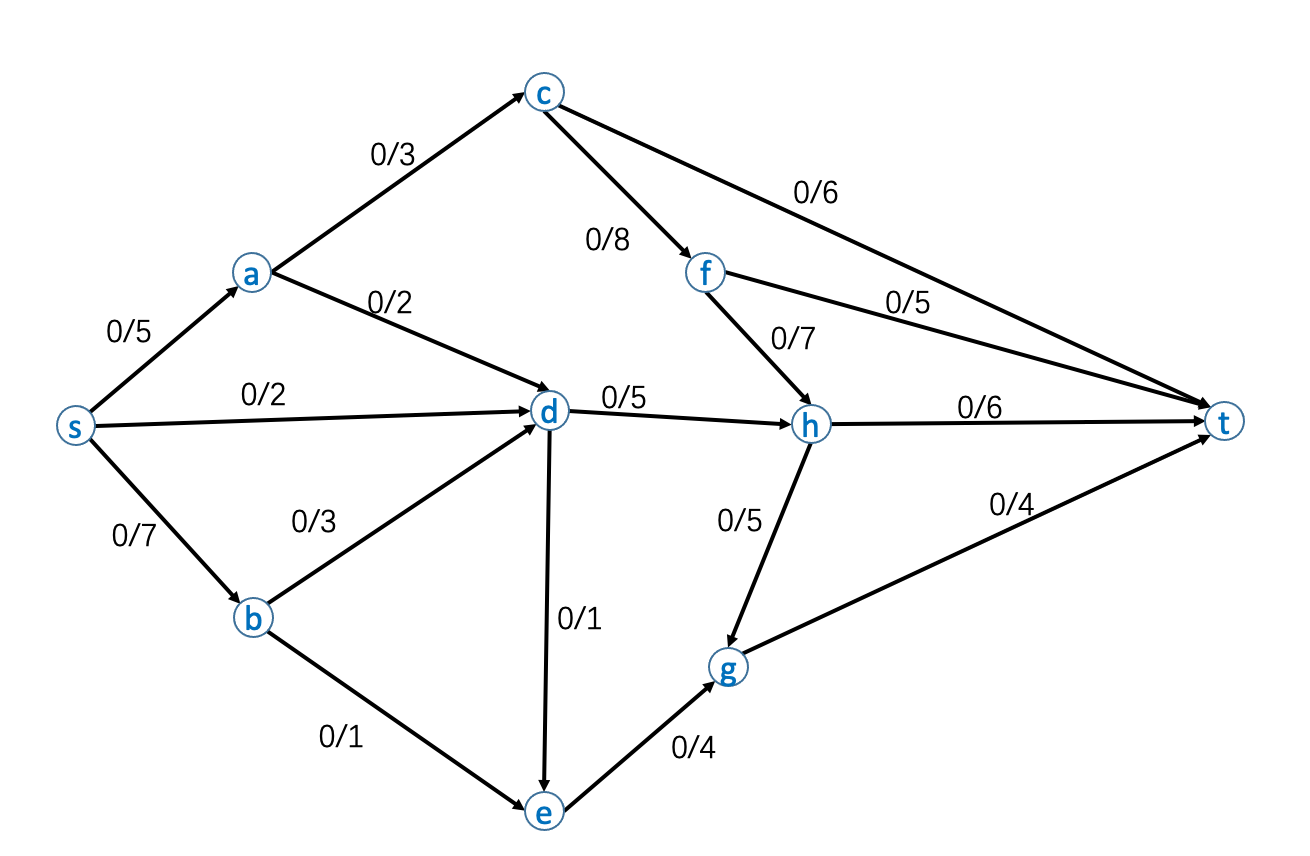
\includegraphics[width=0.8\textwidth]{q5a1}
			\centering
		\end{figure}
		\begin{figure}[h!]
			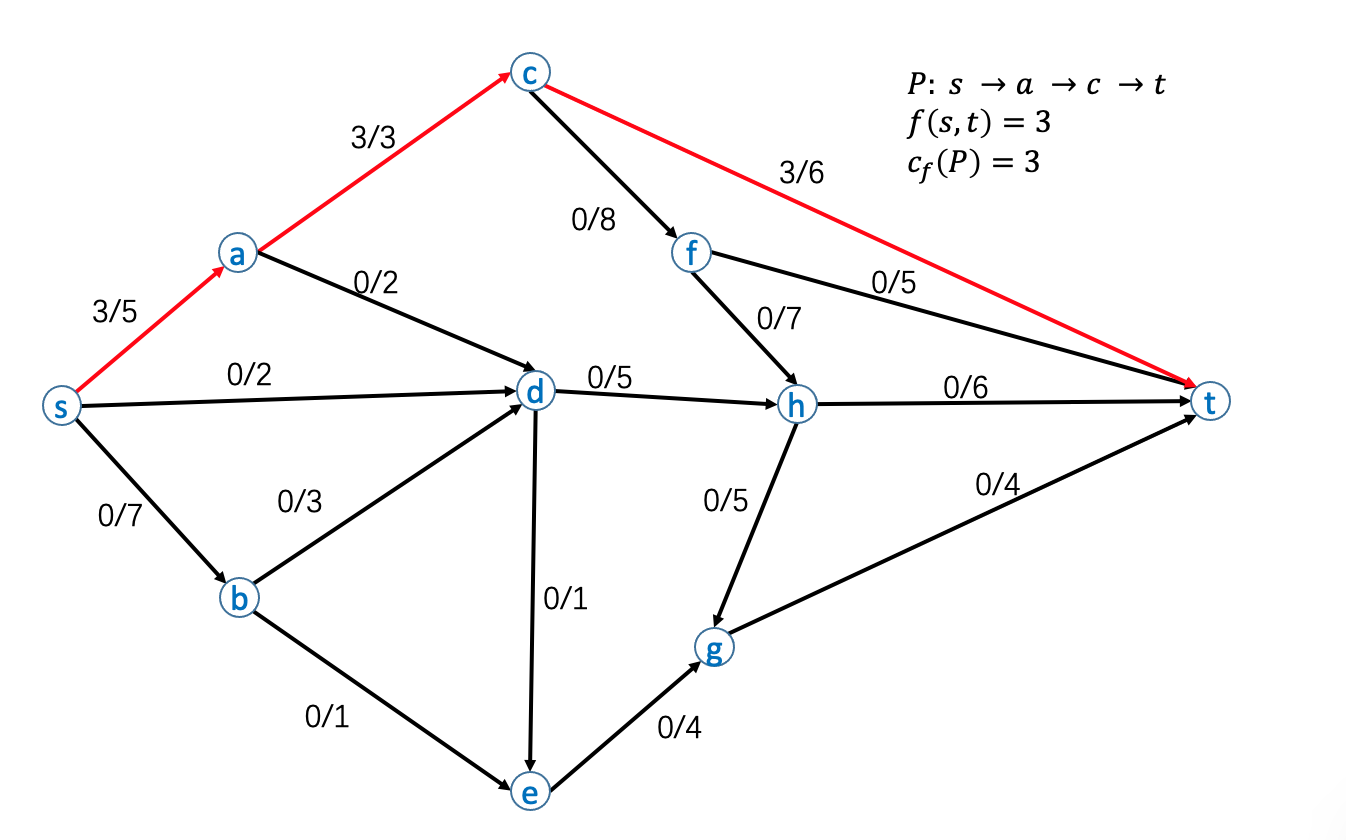
\includegraphics[width=0.8\textwidth]{q5a2}
			\centering
		\end{figure}
		\begin{figure}[h!]
			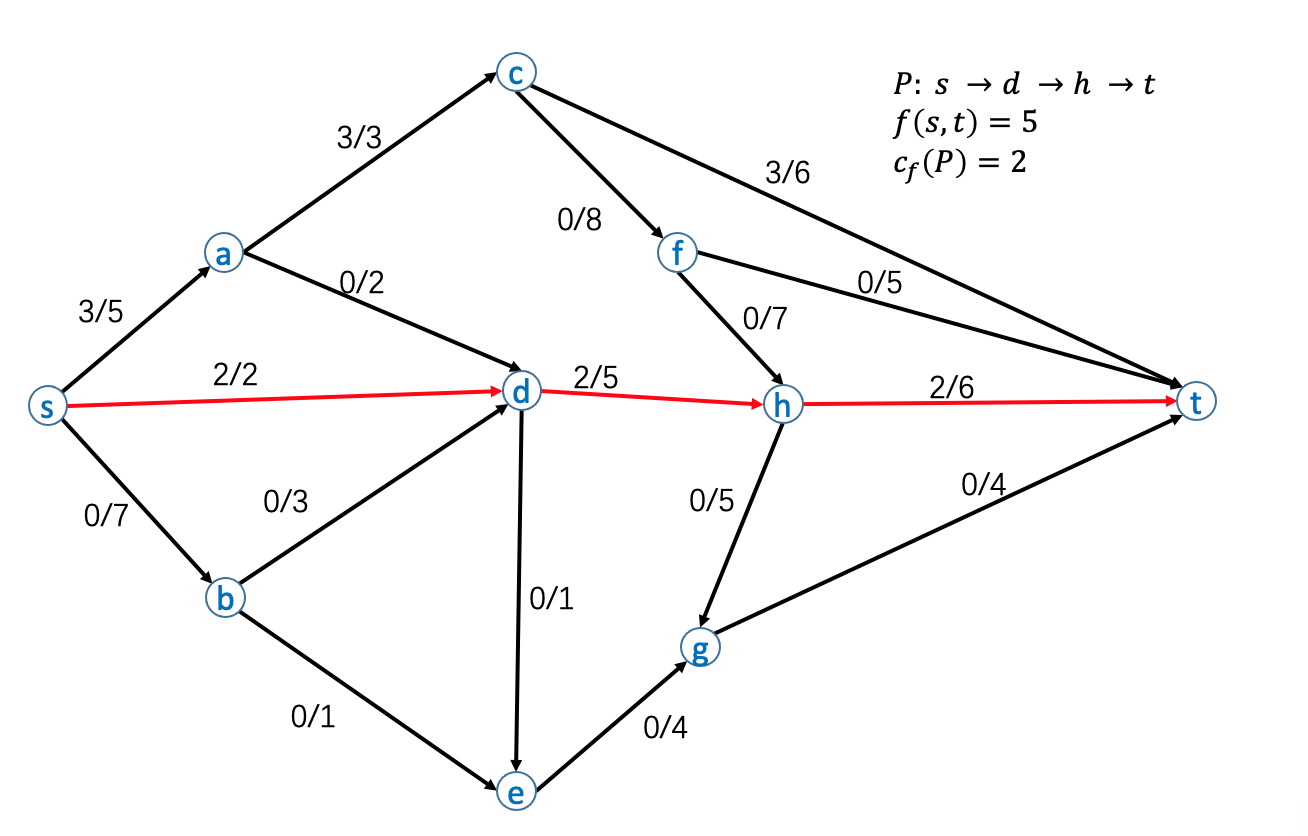
\includegraphics[width=0.8\textwidth]{q5a3}
			\centering
		\end{figure}
		\begin{figure}[h!]
			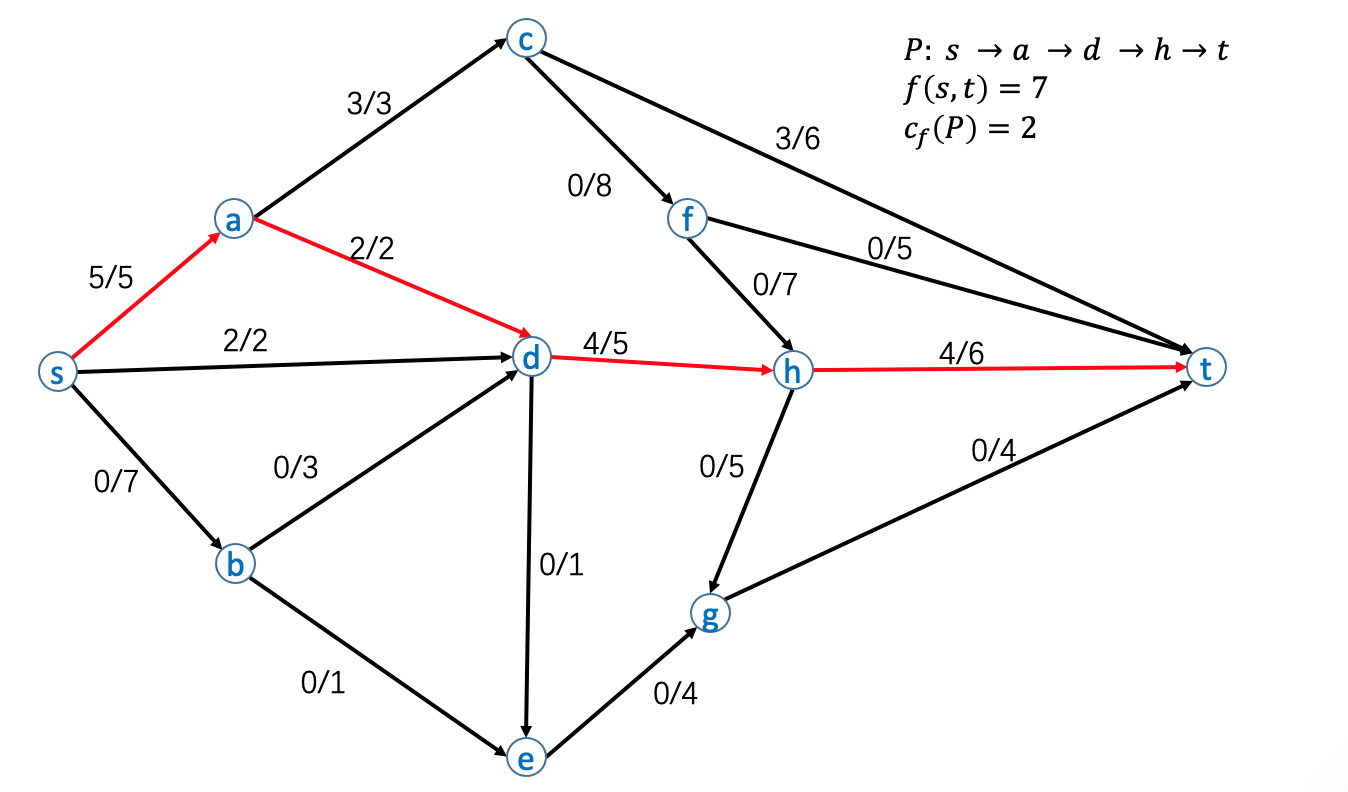
\includegraphics[width=0.8\textwidth]{q5a4}
			\centering
		\end{figure}
		\begin{figure}[h!]
			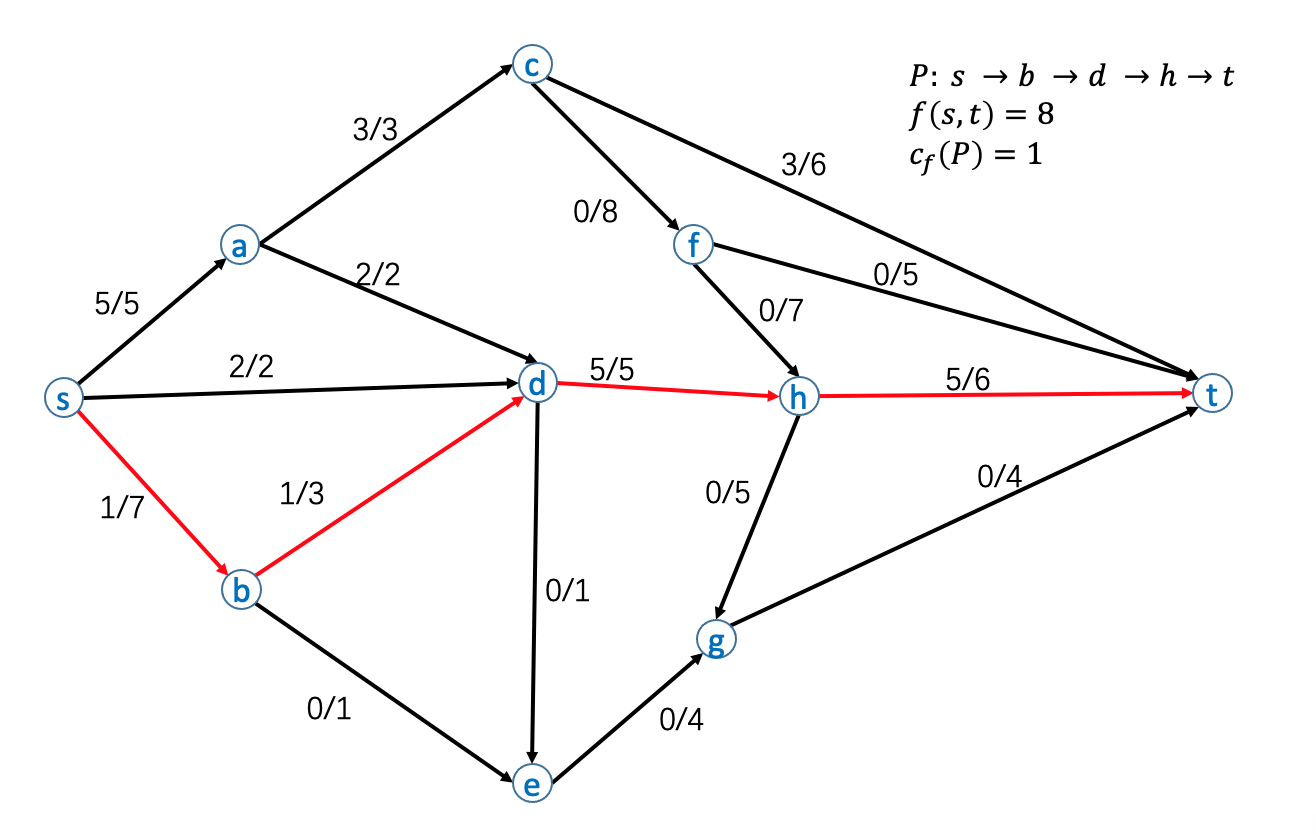
\includegraphics[width=0.8\textwidth]{q5a5}
			\centering
		\end{figure}
		\begin{figure}[h!]
			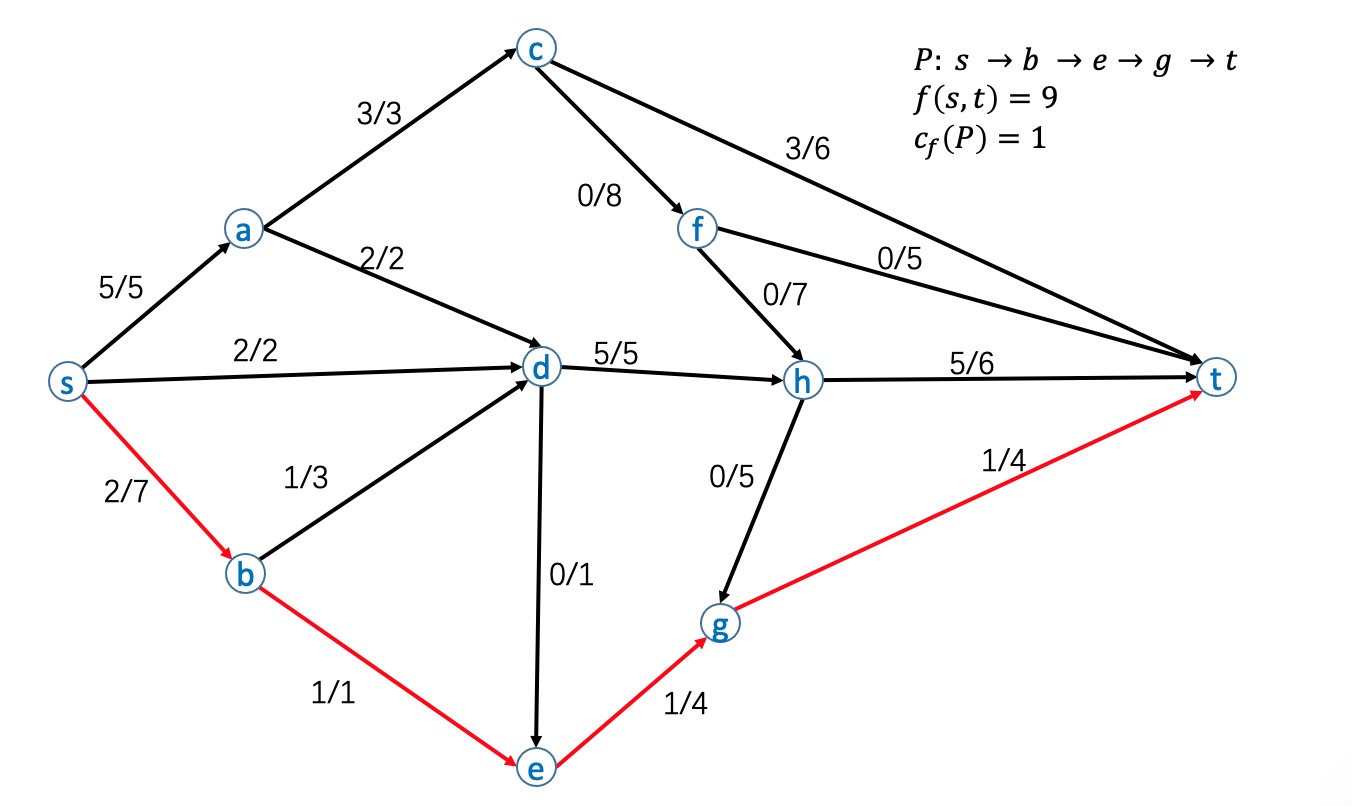
\includegraphics[width=0.8\textwidth]{q5a6}
			\centering
		\end{figure}
		\begin{figure}[h!]
			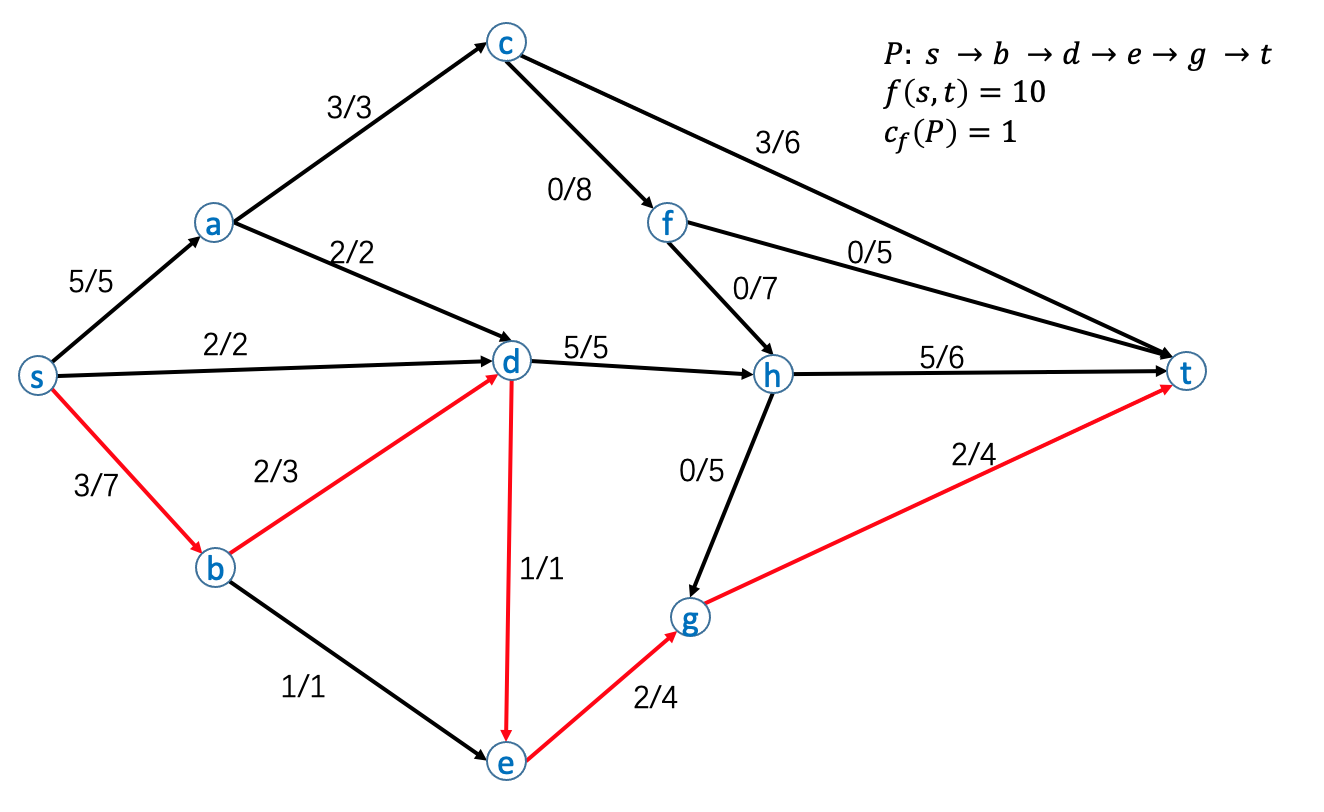
\includegraphics[width=0.8\textwidth]{q5a7}
			\centering
		\end{figure}

		\clearpage
		\newpage
		\item \-
		\begin{figure}[h!]
			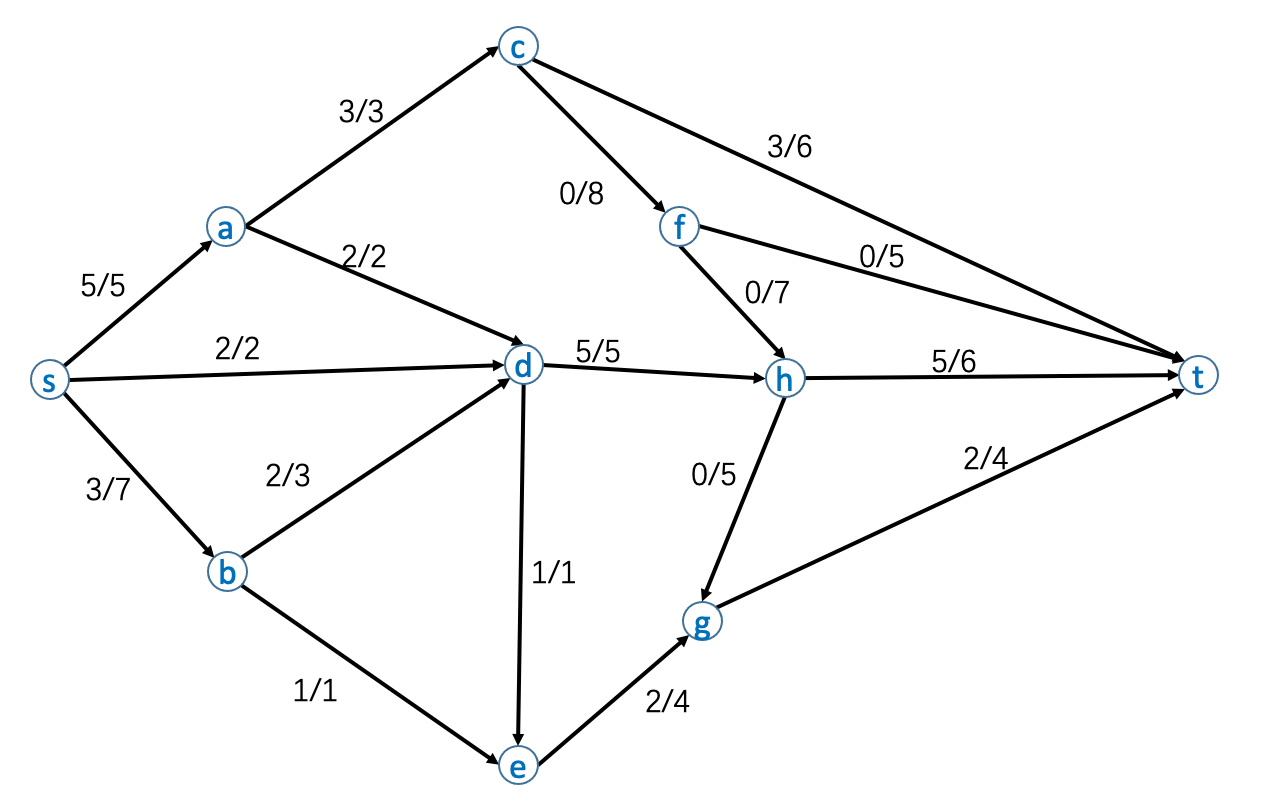
\includegraphics[width=0.8\textwidth]{q5b1}
			\centering
		\end{figure}
		\begin{figure}[h!]
			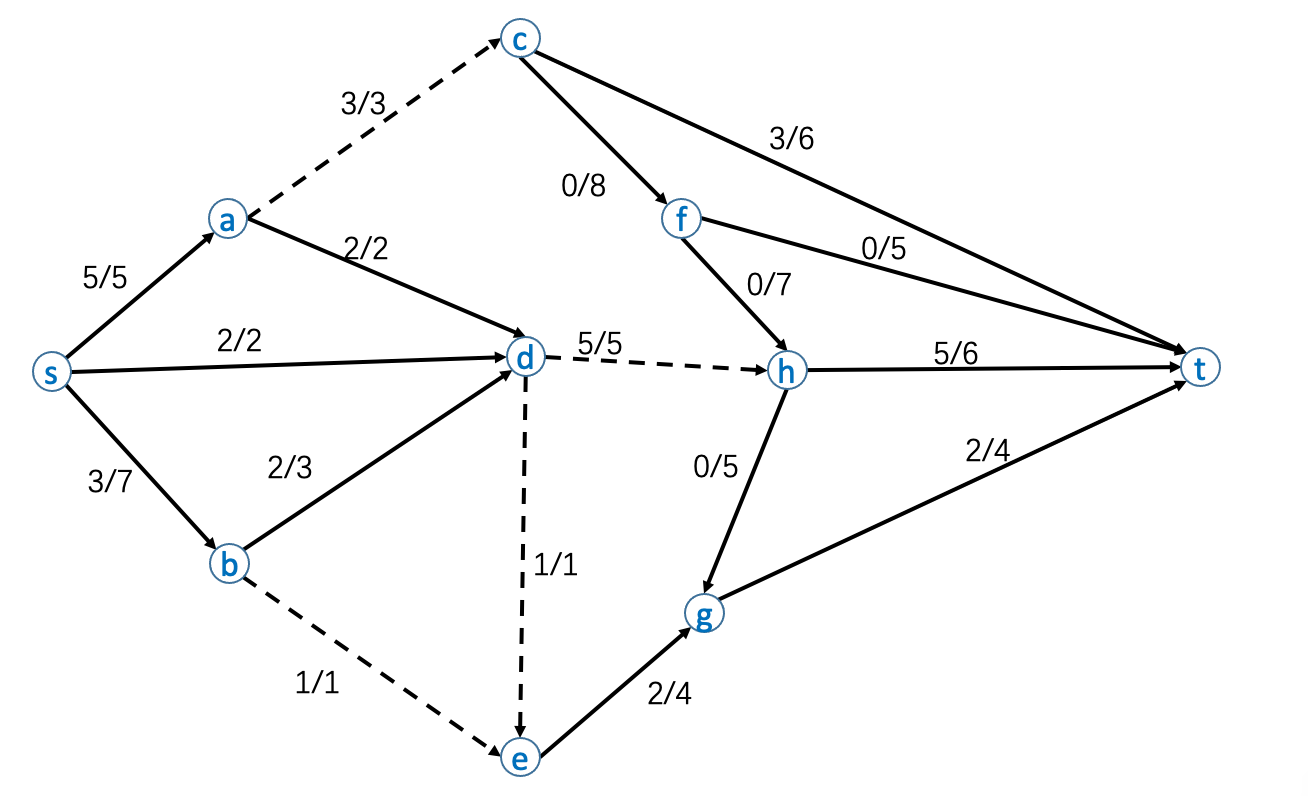
\includegraphics[width=0.8\textwidth]{q5b2}
			\centering
		\end{figure}

	\end{enumerate}
	


\end{document}